\section[Short]{Normas de Elaboração}
    % \subsection{Uma subseção}
    % Aqui temos o conteúdo dessa subseção, referenciando a Seção \ref{sec1}. Em seguida, um comentário. %Isso está comentado.

    O que o projeto deve abordar:
    \begin{itemize}
        \item O que fazer
        \item Por que fazer
        \item Para quem
        \item Onde fazer
        \item Como, com que, quanto e quando fazer
        \item Com quanto fazer e quem vai pagar
        \item Quem vai fazer
    \end{itemize}

    \subsection{Projeto de Pesquisa}

        \indent \textbf{Tema}: definição do que vai ser pesquisado, podendo surgir de situações do cotidiano.

        \textbf{Problema}: consiste em um enunciado explicitado de forma clara, compreensível e operacional, cujo melhor modo de solução é uma pesquisa. Observar: viabilidade, relevância, novidade, exequibilidade e oportunidade. O problema pode ser enunciado em forma de pergunta.

        \textbf{Hipótese}: prováveis respostas, explicações provisórias, afirmações que serão testadas mediante a reflexão teórica ou evidência dos dados. Ao final da pesquisa, as hipóteses podem ser confirmadas ou rejeitadas. Considerada como uma proposição antecipada à comprovação da realidade existencial, deve ter um enunciado claro, conciso, específico, verificável, plausível e relevante. A hipótese é uma tentativa antecipada de responder ao problema.

        \textbf{Justificativa}: é o único item do projeto que apresenta respostas à questão "por que?". Geralmente é o elemento que contribui mais diretamente na aceitação da pesquisa. Pode ser mista: teórica e prática. Se for totalmente de uma forma ou outra, também é válida.

        A pesquisa deve:
        \begin{itemize}
            \item Deve ser interrroativa, clara, precisa e objetiva
            \item Possuir solução viável
            \item Expressar uma relação entre duas ou mais variáveis
            \item Ser fruto de revisão de literatura e reflexão pessoal
        \end{itemize}

        \begin{quotation}
            Inovação é o uso da criatividade com a geração de resultado.
        \end{quotation}

        Importante que as referências sejam publicações.

        Enunciado das hipóteses:
        \begin{itemize}
            \item É uma suposição que se faz na tentativa de explicar o problema;
            \item Como resposta e explicação provisória, relaciona duas ou mais variáveis do problema levantado;
            \item Deve ser testável e responder ao problema;
            \item Serve de guia na pesquisa para verificar sua validade;
            \item Surgem de:
            \begin{itemize}
                \item Observações
                \item Resultados de outras pesquisas
                \item Teorias
                \item Intuição
            \end{itemize}
        \end{itemize}

        Características das hipóteses:
        \begin{itemize}
            \item Consistência lógica
            \item Verificabilidade
            \item Simplicidade
            \item Relevância
            \item Apoio teórico
            \item Especificidade
            \item Clareza
            \item Profundidade
            \item Fertilidade: dali podem surgir novas possibilidades
            \item \textcolor{red}{\textbf{Originabilidade: mais importante para quem vai para o doutorado}}
        \end{itemize}

        \textbf{Objetivos}: determina as metas que queremos alcançar, ou seja, para que pesquisar. Podem ser divididos em gerais (o que queremos alcançar mais amplamente com o desenvolvimento da pesquisa) e específicos (determinam aspectos particulares que se pretendem estudar, compreender, explicar a fim de alcançar o objetivo geral).

        Atenção: o objetivo geral é um só verbo.

        Hipótese é como vai resolver. Objetivo é o que se espera resolver.

        Os objetivos podem ser listado como itens, com verbos de ação no infinitivo (estudar, compreender, endender explicar, saber). Cada objetivo só pode ter um único verbo de ação. Vai ser o último a ser ajustado, depois até das considerações finais. A figura \ref{verbos-objetivos} mostra alguns verbos.

        \begin{figure}[h]
            \centering
            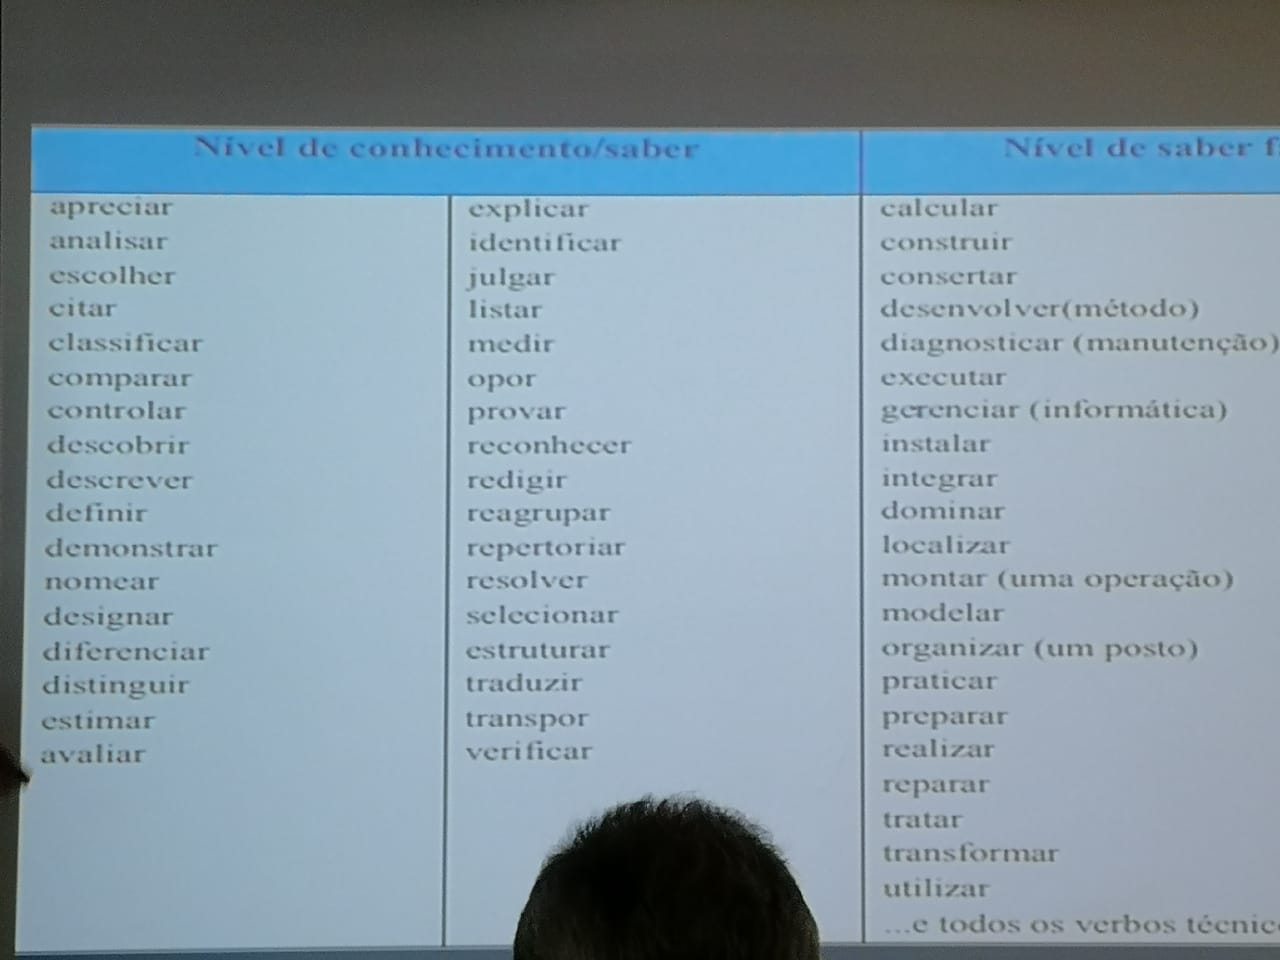
\includegraphics[width=1\textwidth]{verbos-objetivos}
            \caption[Figura]{Verbos usados para os objetivos}
            \label{verbos-objetivos}
        \end{figure}

    % \subsection{Tabelas}
    % Demonstrando uma tabela: \\

    % \begin{tabular}{|l|r|r|} 
    %     \hline
    %     Item & Quantidade & Preço (R\$)\\
    %     \hline
    %     Nails & 500 & 0,34 \\
    %     \hline
    %     Wooden boards & 100 & 4.0 \\
    %     \hline
    % \end{tabular}

    % \subsection{Figuras}
    % Agora veja uma imagem qualquer: \\

    % \begin{figure}[h]
    %     \centering
    %     \includegraphics[width=1\textwidth]{celulares}
    %     \caption[Figura]{Aqui está minha imagem}
    %     \label{imagem-celulares}
    % \end{figure}